\chapter{Privacy}
\label{ch:privacy}

\only<article>{ One interpretation of privacy is simply the ability to
  maintain a personal secret. Is it possible to maintain perfect
  secrecy? Can the thoughts in our head be perfectly safe, or can they
  be revealed indirectly through our actions?

  While we certainly \emph{can} securely store and transmit data using
  cryptography, the problems we will discuss in this chapter are
  \emph{not} solveable solely through cryptography. We are interested
  in scenarios where we must make a public decision or release some
  summary statistics that depend on private data, in such a way as to
  minimise harm to the individuals contributing their data.

  If we never have to reveal any of our computations, cryptography is
  what is needed. For example, through homomorphic computation, an
  untrusted party can even perform some computations on encrypted
  data, returning an encrypted result to us, while learning nothing
  about the original secret.  As long as the data, and the results of
  any computation on it, are kept under lock and key, our personal
  information cannot be revealed.

  However, sometimes we must make public decisions or release
  public information based on this data. Then it can be revealed
  indirectly. For example, you can trust your doctor to maintain
  confidentiality, but when you go to the pharmacy to get the prescribed
  medicine, somebody can infer the medical condition you suffer from.

  It is even possible to learn personal information from aggregate
  statistics.  Let us say your doctor publishes a list of cases of
  different diseases every week, together with some other information
  such as the approximate patient age. Even though your own data is
  mixed with that of all other patients, it is possible to infer your
  diagnosis, especially with some additional side-information: If
  somebody knows you were the only person in that age group visiting
  the doctor that week, they will learn your diagnosis.
  
  From that point of view, it is not the data itself, but the complete
  process of data collection, treatment and public release that can be
  characterised as private or non-private.  For that reason, we will
  emphasise an \emph{algorithmic} view of privacy: participants
  entrusts their data to an algorithm, which produces a useful output
  in return. The algorithmic process is typically not fully automated,
  as it also depends on some human input: One example is a medical
  study examining different treatments for a disease. While humans
  select and administer the treatments, they will typically rely on a
  randomised strategy for assigning treatments to individuals, and use
  a statistical method to report their results.  Given this mixture of
  ad-hoc decisions and formal algorithmic methods, is it possible to
  guarantee privacy in any sense? What kind of guarantees can we make?

  Generally speaking, an algorithm has good privacy properties, if the
  amount of information that can be revealed through the algorithm's
  output about any individual contributing data is bounded. In
  particular, we are interested in how much an adversary can learn
  about any individual's input to the algorithm from the algorithm's
  output.

  This does not preclude learning general facts about individuals from
  the output. For example, a study about the use of steroids in sports
  may show that 90\% of sprinters with times under 10 seconds are
  using steroids, while only 50\% of slower sprinters do so. Any
  sprinter with a time under 10 seconds is thus suspected of using
  steroids by association. However, it does not matter if their data
  has been used in the study. The publication of the result does not
  impact their privacy, but the amount of harm it does to them does
  not depend in their participation: the same statistical result would
  have been obtained with or without them.
  
  In this chapter, we will look at two formal concepts of privacy
  protection: $k$-anonymity and \emph{differential privacy}. The first
  is a simple method for anonymising databases. However, it provides
  only limited resistance to identification. The latter is a more
  general concept, which provides full information-theoretic
  protection to individuals. A major problem with any privacy
  definition and method, however is correct interpretation of the
  privacy concept used, and correct implementation of the algorithm
  used.
}

\section{Algorithmic privacy.}
\begin{frame}
  \frametitle{What is an algorithm?}
  \only<article>{Any functional process is an algorithm. We typically
    identify inputs with observations or features $\CX$, and outputs
    with actions $\CA$ by the algorithm: i.e. we view the algorithm as
    taking actions that have an observable effect on its external
    environment. We generally consider \emph{stochastic} algorithms.}
  \begin{definition}[Stochastic algorithm $\pi$]
    A stochastic algorithm $\pi$ with input domain $\CX$ and output
    domain $\CA$ is a mapping $\pi : \CX \to \Simplex(\CA)$ from
    observations $\CX$ to distributions over outputs
    $\Simplex(\CA$). When $\CA$ is finite, we will write
    $\pol(a \mid x)$ to denote the conditional probability that the
    algorithm outputs $a$ given input $x$.
  \end{definition}
  \only<article>{
    \begin{theoryblock}{The general case.}
      It is best to think of $\pol(\cdot | x)$ as a probability
      measure over $\CA$. Then we write
      \[
        \pol(A \mid x) \defn \Pr_\pol(a \in A \mid x), \qquad A \subset \CA,
      \]
      for the conditional probability that algorithm's output is in
      some set $A \subset \CA$ given input $x$. This allows us to treat
      the case when $\CA$ is continuous or discrete with the same notation.
    \end{theoryblock}
    
    \begin{exampleblock}{Algorithmic randomness.}
      We can construct a random algorithm through access to a random
      coin $\omega$ taking values in $\Omega$. We can then define the
      output through a deterministic function $a_\pi(\omega, x)$. Since
      $\omega$ is random, the output of the function is also random.
      If $P$ is the probability distribution of $\omega$, then:
      \[
        \pi(A \mid x) = P(\cset{\omega \in \Omega}{a_\pi(\omega, x) \in A}),
      \]
      i.e. the probability that the algorithm's output is in $A$ is
      equal to the measure of the values of $\omega$ for which the
      $a_\pi(\omega, x) \in A$.
    \end{exampleblock}
  }
\end{frame}

\begin{frame}
  \begin{figure}
    \centering
    \includegraphics[height=\fheight]{../figures/smbc-the-problem}
    % Copyright: SMBC
  \end{figure}
\end{frame}
\begin{frame}
  \frametitle{Privacy in statistical disclosure.}
  \only<article>{ Fundamentally, privacy in statistics is an \emph{issue of
      trust.} The analyst, be it a human, or an automated service, will
    use your data to make decisions. You must also decide who to trust
    and how much. Do we trust the data analyst? How much privacy are
    we willing to sacrifice to the analyst? How much to the public at
    large?  What you want out of the service.  Is the service
    important enough to sacrifice significant amounts of privacy? What
    is an acceptable trade-off between utility and privacy?  These are
    difficult questions and are hard to quantify, hence we assume that
    we have already decided how to answer them, and we simply want to
    find an appropriate methodology for achieving a good result.  }
  
  \only<presentation>{
    \begin{block}{An issue of trust}
      \begin{itemize}
      \item Who to trust and how much.
      \item What you want out of the service.
      \end{itemize}
    \end{block}
  }

  \only<article>{ Consider a researcher wishing to collect data for a  statistical analysis. As long as the analysis is eventually
    published,\footnote{If somebody knows that the analysis is being
      conducted, however, they could still learn something private from the fact that the analysis has \emph{not} been published.} this
    creates two possible scenarios for that may lead to privacy violations.}
  \begin{itemize}
  \item Publication of ``anonymised'' data.
    \only<article>{Sometimes we may collect data in order to publish the dataset itself for other researchers to use. This is common practice in machine learning, with image classification datasets being a good example. However, if the data contains personal information, there is always some privacy risk even if the data has been anonymised with standard methods.}
  \item Public data analysis. \only<article>{This is a more general setting, where we never publish individual data records, but only summary statistics or models about the data. A prime example is a national census analysis, which may provide detailed demographic information for all towns and regions in a nation. Although only aggregate data is published, it is theoretically possible to infer personal information. For that reason, the US Census Bureau conducted its analysis in 2020 using differential private algorithms.}
  \end{itemize}
  \begin{alertblock}{Cryptography is not enough.}
    \only<article>{ Cryptography provides:}
    \begin{itemize}
    \item Secure communication and computation.
    \item Authentication and verification.
    \end{itemize}
    \only<article>{These are useful to establish secure channels with somebody that we trust. However, the privacy violations we are concerned with relate to \alert{publicly released} outputs of algorithms. It is not important whether or not all the data and computation are encrypted: as long as the algorithm generates a public output, it is theoretically possible for somebody to learn something about the algorithm's input.}
  \end{alertblock}


\end{frame}

\section{Things we do with data}
\only<presentation>{
\begin{frame}
  \begin{block}{Reasons for data collection}
    \begin{itemize}
    \item To publish it.
    \item To publish specific statistics.
    \item To make decisions through arbitrary computations.
    \end{itemize}
  \end{block}
\end{frame}
} \only<article>{ How do we use data in the first place? Sometimes we
  simply publish the data, perhaps after some initial
  processing. Publication of datasets is useful for researchers that
  want to do perform further analysis on the data. Usually though, we collect data in order to calculate specific statistics. For example the census collects data about the number of people in different households, wages, etc, and then publishes tables detailing the average age and number of people per household in different areas of the country. This demographic information is useful for policy makers, urban planning to organise voting centers and the distribution of police and fire stations, as well as other public services. }
\section{Statistical disclosure}

\only<presentation>{
  \begin{frame}
    \tableofcontents[ 
    currentsection, 
    hideothersubsections, 
    sectionstyle=show/shaded
    ] 
  \end{frame}
}

\only<article>{
  \begin{centering}
    \emph{``Data is everywhere'', said the statistician, ``data, data!''.}
  \end{centering}

  In the past, statistical analysis was performed
  with laboriously collected and annotated datasets. Even as
  recently as in the early 21st century, databases for machine
  learning were limited to a few thousand entries at most. At the
  time of writing, not only has the size of datasets become
  extremely large, but the sources of data are much more
  diverse. Data are collected and commercialised whenever we visit a
  website and even as we walk around with our phone. To a limited
  extent, there is a tradeoff between what we can get out of a
  service and what we pay into it. Many free services such as
  navigation software rely on collecting user data to perform
  better: If you can tell that there is a traffic jam in Central
  Avenue, you can after all try and take another route.  As long as
  informed consent exists, use of private data is generally regarded
  as unproblematic.\footnote{This is actually underscored by the
    GDPR legislation, which focuses on consent and data use
    methods.}

  However, even apparently benign data collected with appropriate
  consent can lead to serious and unexpected privacy
  violations. There are three famous examples of this: Firstly, the
  identification of people in supposedly anonymous health data in
  the 1990s in the state of Massachussets, which we will go over in
  detail in this chapter. Secondly, the identifications of users
  through anonymised movie ratings in the Netflix dataset. Finally,
  the ability to discover if any given individual's data is
  contained in a pooled genomic study.
}
\begin{frame}
  \frametitle{Anonymisation}
  \only<article>{Data is collected for many reasons. Any typical service you might want to use will require a minimal amount of data. For example, a dating service will at a minimum require your age and location, as shown in the example below.}
  \begin{example}[Typical relational database in a dating website.]
    \begin{table}[H]
      \begin{tabular}{l|l|l|l|l|l|l}
        Birthday & Name & Height  & Weight & Age & Postcode & Profession\\
        \hline
        06/07 & \only<1>{Li Pu} & 190 & 80 & 60-70 & 1001 & Politician\\
        06/14 & \only<1>{Sara Lee} & 185 & 110 & 70+ & 1001 & Rentier\\
        01/01 & \only<1>{A. B. Student} & 170 & 70 & 40-60 & 6732 & Time Traveller
      \end{tabular} 
    \end{table}
    \only<article>{ If somebody is a user in a dating website, you
      expect them to give some minimal personal information to be
      stored in the site's database. This might include their
      birthday, location and profession, for example.} 
  \end{example}
  \only<article>{When you submit your data to a service, you expect it to be used responsibly. For the dating service, you expect it to use the information to find good matches, based on your preferences and location. Whenever somebody uses the service, they obtain some information about you, at least indirectly. For example, if they make a query for similar singles in their neighbourhood, and they see your profile, then they have learned that you live nearby.

    If we wish to publish a database, frequently we need to protect identities of people involved. The simplest method for doing that is simply erasing directly identifying information. However, this does not really work most of the time, especially since attackers can have side-information that can reveal the identities of individuals in the original data.
  }
  
  \only<2>{The simple act of hiding or using random identifiers is called anonymisation.}
  \only<article>{However this is generally insufficient as other identifying information may be used to re-identify individuals in the data.}
\end{frame}


\begin{frame}
  \frametitle{Record linkage}
  \only<article>{
    In particular, even if somebody is unable to infer the information of any individual from the published, anonymised, dataset, they may be able to do so via some side-information. All that is needed is another dataset with some columns in common with the dataset they want to target.

    As an example, in the 1990s a the governor of Massachussets,
    decided to publish anonymised information about the health records
    of individual state employs. They were careful to hide all
    obviously identifying information such as their name, and thus
    claimed that there are no potential privacy violations. However,
    they left in some information that they thought would be useful
    for researchers: the postcode, the birthdate, and the sex of each
    individual.

    This allowed a PhD student, McSweeney, to perform the following
    linkage attack. She order a floppy disk containing database of
    voting records in the state. This contained names and addresses,
    as well as the postcode, birthdate and sex of every voter. In that
    way, she was able to cross-reference this data, and so obtain the
    identities of individuals in that database. The first record she
    obtained was that of the governor himself, Bill Weld. Later, she
    estimated that approximately 87\% of Americans are uniquely
    identifiable through those three attributes.

    Clearly, anonymisation is not enough. So, is there a way to
    formally guarantee privacy? In the next section we will go over
    the solution of McSweeny, which is sadly insufficient to protect
    privacy in general. Later, we will introduce the notion of
    differential privacy, which protects individuals against
    statistical disclosure in an information-theoretic manner.

  }

  \begin{columns}
    \begin{column}{0.7\textwidth}
      \centering \def\firstcircle{(0,0) circle (7em)}
      \def\secondcircle{(3,0) circle (7em)}
      
      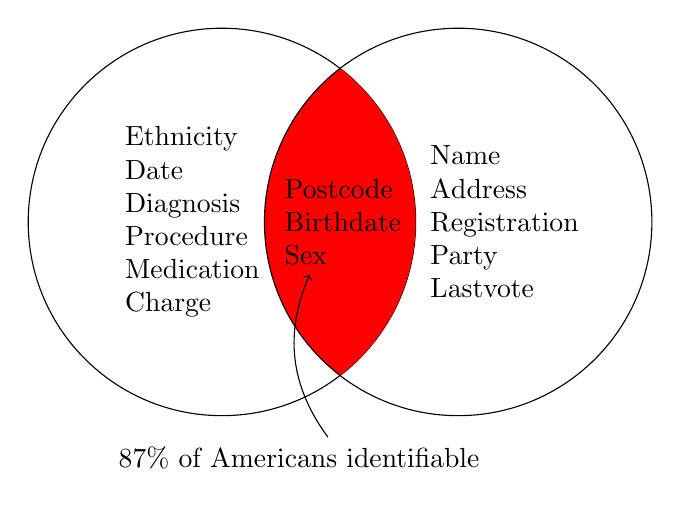
\begin{tikzpicture}
        \uncover<1,3>{ \draw \firstcircle node[text width=7em]
          {Ethnicity\newline Date\newline Diagnosis \newline Procedure
            \newline Medication \newline Charge }; } \uncover<3>{
          \begin{scope}
            \clip \firstcircle; \fill[red] \secondcircle;
          \end{scope}
        } \uncover<2,3>{\draw \secondcircle node [text width=2em,
          align=right] {Name \newline Address \newline Registration
            \newline Party \newline Lastvote}; } \node [text width=4em]
        (QI) at (1.5, 0) {Postcode \newline Birthdate \newline Sex};
        \uncover<3>{ \node [text width=16em] (qi-text) at (1.5, -3)
          {87\% of Americans identifiable}; \path[->]<1-> (qi-text) edge [bend left]
          (QI); }
      \end{tikzpicture}
    \end{column}
    \begin{column}{0.3\textwidth}
      \includegraphics[height=\fheight]{../figures/Bill_Weld}
      \\
      Bill Weld, R-MA
    \end{column}
  \end{columns}
\end{frame}

\begin{frame}
  \begin{example}[Typical relational database in a tax office]
    \begin{table}[H]
      \begin{tabular}{l|l|l|l|l|l|l}
        ID & Name &  Salary & Deposits & Age & Postcode & Profession\\
        \hline
        1959060783 & Li Pu & 150,000 & 1e6 & 60 & 1001 & Politician\\
        1946061408 & Sara Lee & 300,000 & -1e9 & 72 & 1001 & Rentier\\
        2100010101 & A. B. Student & 10,000 & 100,000 & 40 & 6732 & Time Traveller
      \end{tabular}
    \end{table}
  \end{example}
\end{frame}

% \begin{frame}
%   \frametitle{Data linkage with SQL}
%   The original database \verb|database| and adversary side information \verb|side-information| can be combined using the following simple SQL query:
% \begin{verbatim}
% SELECT * FROM database JOIN side-information ON [condition]
% \end{verbatim}
%   where \verb|condition| describes how to match the records.

%   \begin{example}
%     For the databases given above, we could use
% \begin{verbatim}
% SELECT * FROM tinder JOIN tax ON tinder.height = tax.height AND tinder.age = tax.age
% \end{verbatim}
%     to create a joint table.
%   \end{example}
% \end{frame}

\section{$k$-anonymity}
\label{sec:k-anonymity}
\begin{frame}
  \frametitle{$k$-anonymity}
  \begin{figure}[H]
    \centering
    \begin{subfigure}{0.45\textwidth}
      \centering
      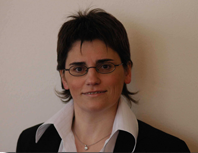
\includegraphics[width=0.9\fwidth]{../figures/samarati}
      \caption{Samarati}
    \end{subfigure}
    \hspace{0.05\textwidth}
    \begin{subfigure}{0.45\textwidth}
      \centering
      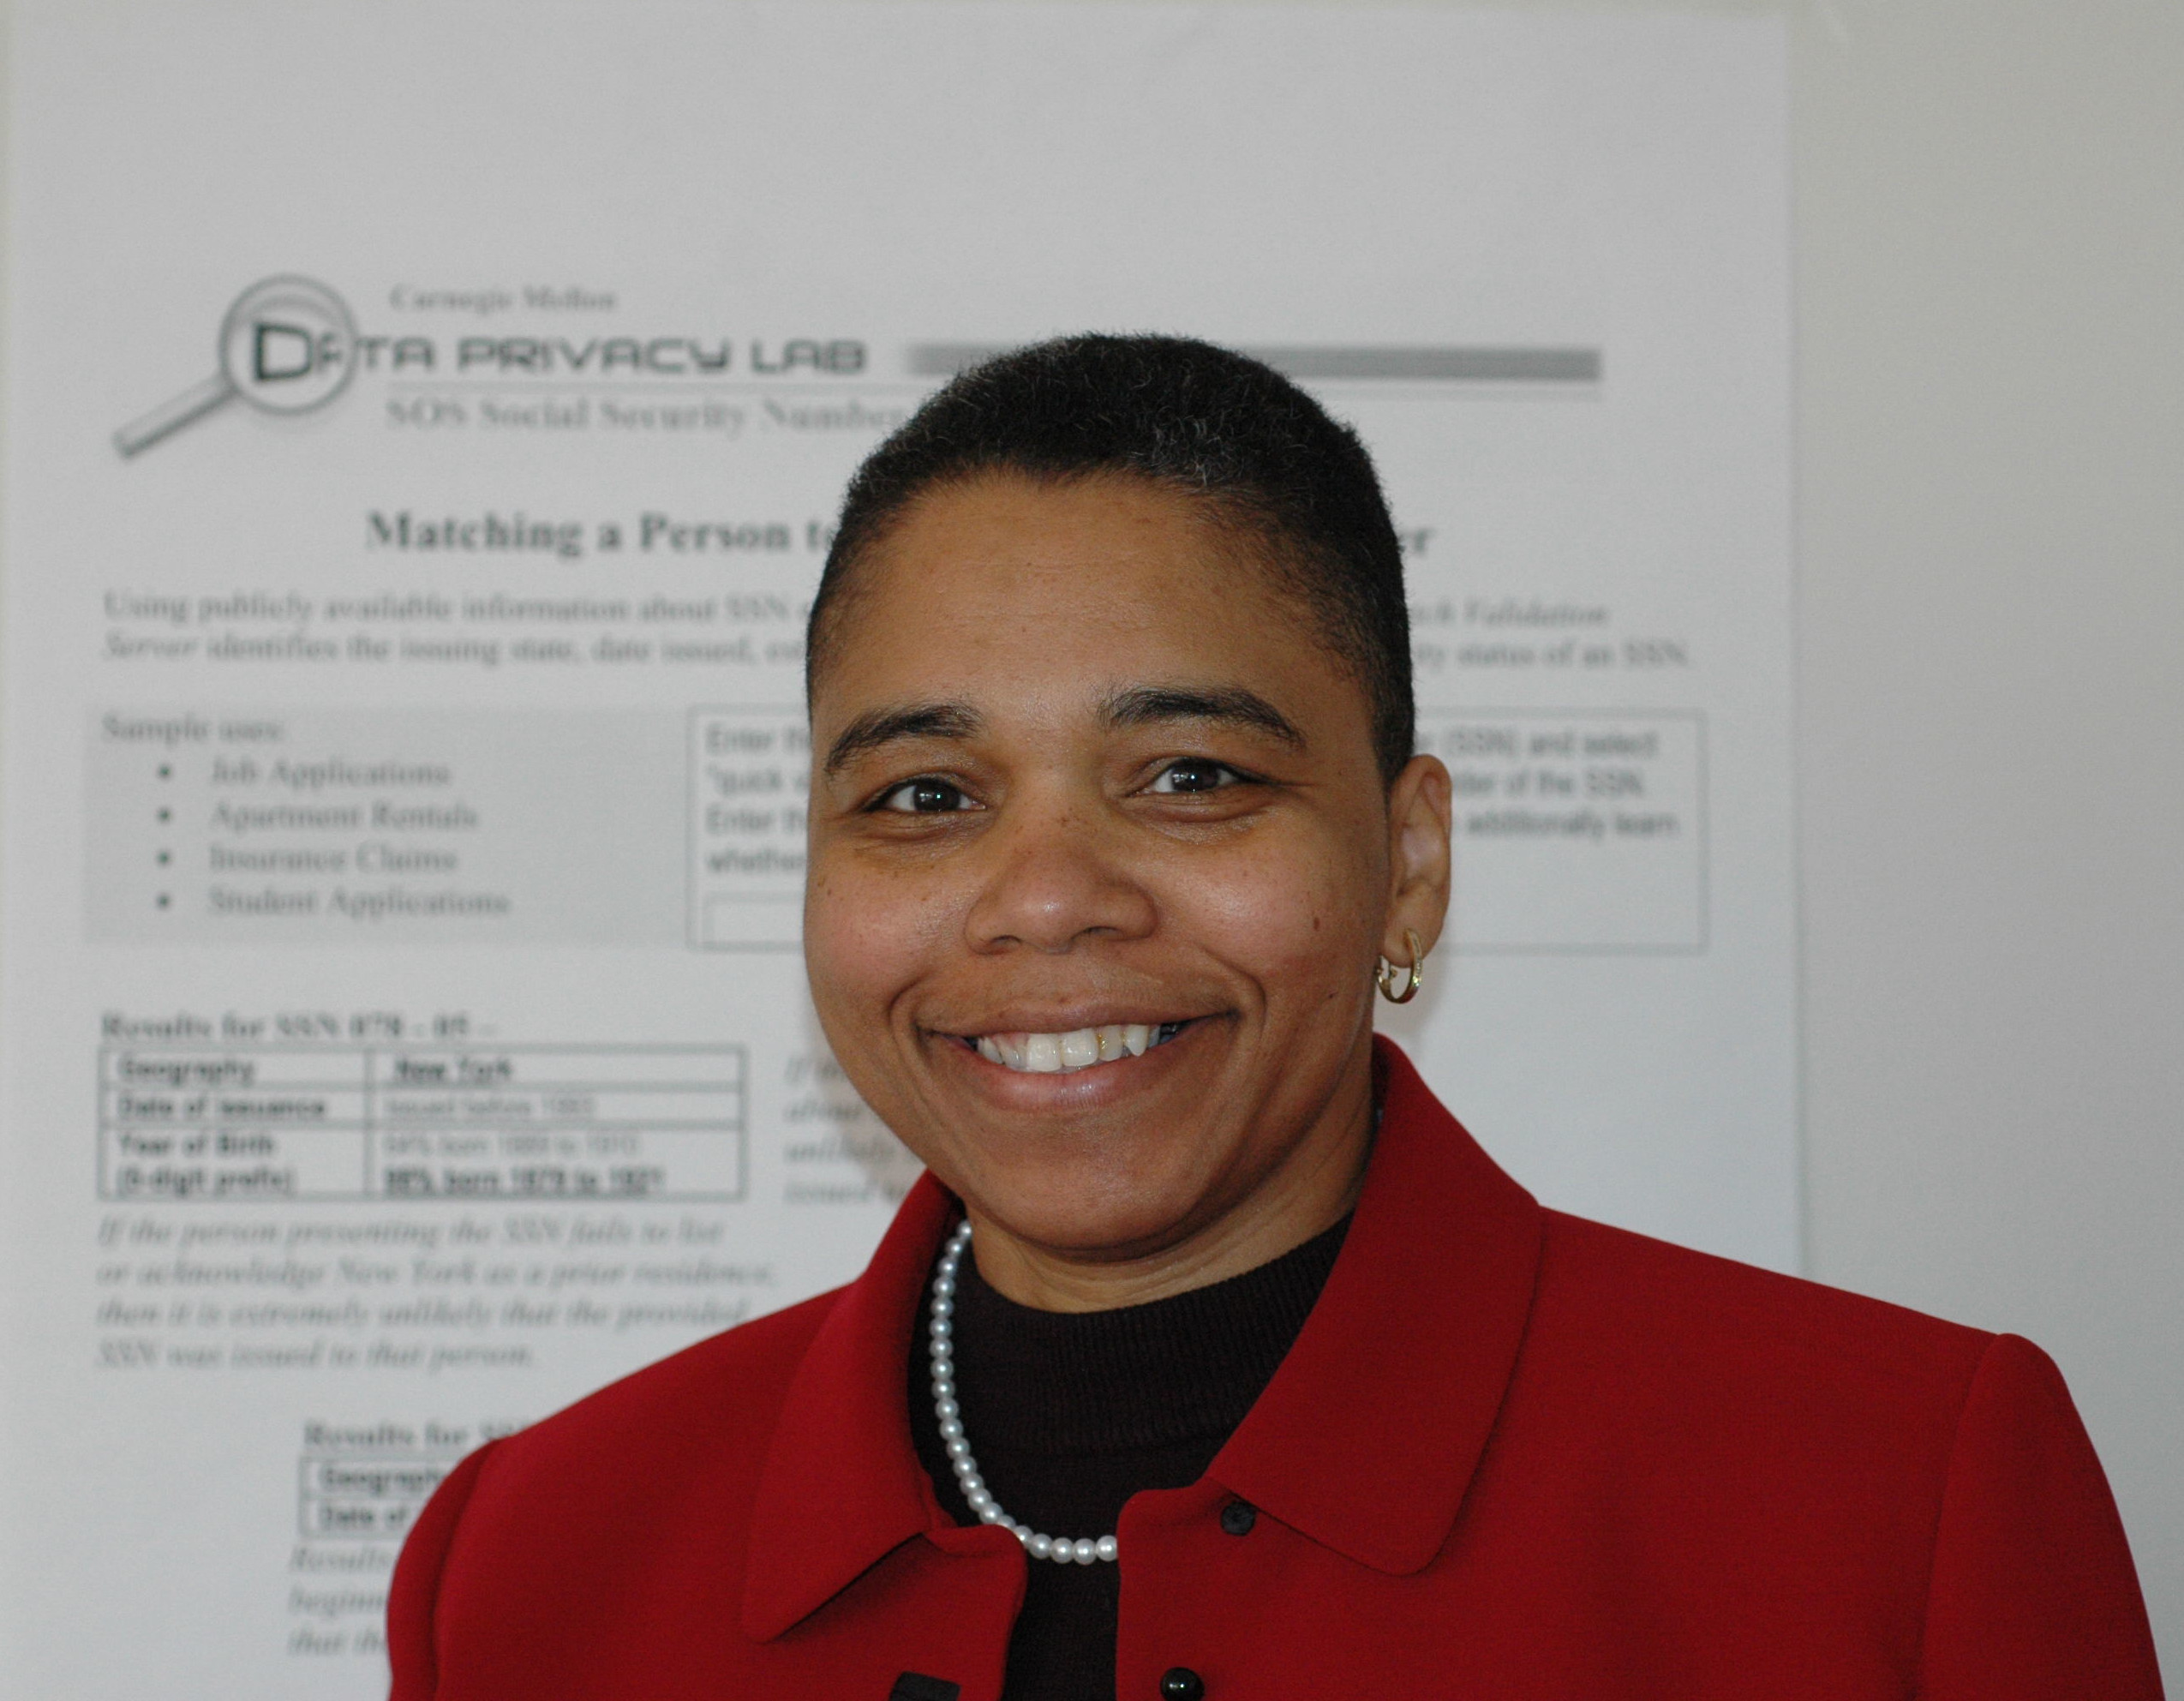
\includegraphics[width=0.9\fwidth]{../figures/sweeney}
      \caption{Sweeney}
    \end{subfigure}
  \end{figure}
  \only<article>{The concept of $k$-anonymity was introduced
    by~\citet{samarati1998protecting} and provides good guarantees
    against inferring personal information from a single
    database. This requires the analyst to first determine the
    variables of interest, and then determine which variables could be
    potentially used to identify somebody in the database.}
  \alert{It's the analyst's job to define quasi-identifiers.}
  \begin{definition}[$k$-anonymity]
    A database provides $k$-anonymity if for every person in the
    database is indistinguishable from $k-1$ persons with respect to
    \emph{quasi-identifiers}.
  \end{definition}
  \only<article>{This hope is that, if the database satisfies
    $k$-anonymity it can be safely released, without revealing any
    private information directly. Let us now walk through an extended
    example.}
\end{frame}

\begin{frame}
  \frametitle{$k$-anonymity example}
  \only<article>{
    In particular, let us say that the analyst simply wants to calculate some statistics about how different professions correlate with age, weight, height and where people live. Some areas of the country might produce more politicians, for example. And taller people may be more successful in politics. The initial data collected might look like the table below. It was obvious to the analyst, that even if he did remove all the names, somebody knowing where A. B. Student lived and saw the table would have little trouble recognising them.
  }

  \only<1>{
    \begin{table}[H]
      \centering
      \begin{tabular}{l|l|l|l|l|l|l}
        Birthday & Name & Height  & Weight & Age & Postcode & Profession\\
        \hline
        06/07 & Li Pu & 190 & 80 & 65 & 1001 & Politician\\
        06/14 & Sara Lee & 185 & 110 & 67 & 1001 & Rentier\\
        06/12 & Nikos Karavas & 180 & 82 & 72+ & 1243 & Politician\\
        01/01 & A. B. Student & 170 & 70 & 52 & 6732 & Time Traveller\\
        05/08 & Li Yang & 175 & 72 & 35 & 6910 & Politician
      \end{tabular}
      \caption{1-anonymity.}
    \end{table}

  }
  \only<presentation>{
    \only<2>{
      \begin{tabular}{l|l|l|l|l|l|l}
        Birthday & Name & Height  & Weight & Age & Postcode & Profession\\
        \hline
        06/07 &  & 190 & 80 & 60+ & 1001 & Politician\\
        06/14 &  & 185 & 110 & 60+ & 1001 & Rentier\\
        06/12 &  & 180 & 82 & 60+ & 1243 & Politician\\
        01/01 &  & 170 & 70 & 40-60 & 6732 & Time Traveller\\
        05/08 &  & 175 & 72 & 30-40 & 6910 & Politician
      \end{tabular}
      1-anonymity
    }

    \only<3>{
      \begin{tabular}{l|l|l|l|l|l|l}
        Birthday & Name & Height  & Weight & Age & Postcode & Profession\\
        \hline
        06/07 &  & 180-190 & 80+ & 60+ & 1* & Politician\\
        06/14 &  & 180-190 & 80+ & 60+ & 1* & Rentier\\
        06/12 &  & 180-190 & 80+ & 60+ & 1* & Politician\\
        01/01 &  & 170-180 & 60-80 & 20-60 & 6* & Time Traveller\\
        05/08 &  & 170-180 & 60-80 & 20-60 & 6* & Politician
      \end{tabular}
      1-anonymity
    }
  }

  \only<article>{After thinking about it for a bit, the analyst decides to remove the birthday and name, and broadly categorise people according to their height in increments of 10cm, the weight in increments of 20cm, and keep just the first digit of the postcode. Now that looked much more reasonable. Still, somebody that knows that Li Yang and A. B. Student are in the table, as well as their postcodes, and they also know that Li Yang is a politician, can infer that A. B. Student is a Time Traveller.}
  \only<4>{
    \begin{table}[H]
      \centering
      \begin{tabular}{l|l|l|l|l|l|l}
        Height  & Weight & Age & Postcode & Profession\\
        \hline
        180-190 & 80+ & 60+ & 1* & Politician\\
        180-190 & 80+ & 60+ & 1* & Rentier\\
        180-190 & 80+ & 60+ & 1* & Politician\\
        170-180 & 60-80 & 20-60 & 6* & Time Traveller\\
        170-180 & 60-80 & 20-60 & 6* & Politician
      \end{tabular}
      \caption{2-anonymity: the database can be partitioned in sets of at least 2 records}
    \end{table}
  }


  \only<article>{However, with enough information, somebody may still
    be able to infer something about the individuals. In the example
    above, it remains true that if somebody knows that both
    A. B. Student and Li Yang are in the database, as well as their
    postcodes, as well as that Li Yang is a politician, they can infer
    A. B. Student's profession.

    Fortunately, there is a way to protect individual information from
    adversaries with arbitrary side-information. This is given by
    differential privacy.
  }
\end{frame}



\section{Differential privacy}
\label{sec:differential-privacy}
\only<article>{ This section introduces one of the main tools for
  giving formal guarantees about the privacy of any algorithm ran on
  a dataset, \emph{differential privacy}. This will provide
  individual-level privacy, in the sense that an algorithm that is
  differentially private guarantees that no adversary can
  significantly increase their knowledge about any particular
  individual by observing the algorithm's output. This is
  independent of the adversary's existing knowledge, or
  computational power. }

\only<article>{While $k$-anonymity can protect against specific
  re-identification attacks when used with care, it says little about
  what to do when the adversary has a lot of knowledge. For example,
  if the adversary knows the data of everybody that has participated
  in the database, it is trivial for them to infer what our own data
  is. For some particularly sensitive datasets, we may want for the
  adversary to be unable to tell whether or not your data was part of
  the base. Differential privacy offers protection against adversaries
  with unlimited side-information or computational power. Informally,
  an algorithmic computation is differentially-private if an adversary
  cannot distinguish two ``neighbouring'' database based on the result
  of the computation. Informally, two databases are neighbours when
  they are identical apart from the data of one person. A
  differentially private algorithm, because of its randomness, makes
  it impossible for somebody to tell from the algorithm's output
  whether any specific individual's data was in the database. }

\begin{frame}
  \begin{figure}[H]
    \centering
    \begin{tikzpicture}[node distance=0.4\textwidth]
      \node[label=left:$x$] at (0,0) (data) {\includegraphics[width=0.1\columnwidth]{../figures/medical}};

      \node[label=$x_1$] at (-2,3)(patient1) {\includegraphics[width=0.05\columnwidth]{../figures/me-recent}};
      \uncover<3->{
        \node[label=$x_2$] at (2,3) (patient2) {\includegraphics[width=0.1\columnwidth]{../figures/judge}};
      }
      \uncover<4->{
        \node[label=$a$] at (4,0)   (statistics) {\includegraphics[width=0.2\columnwidth]{../figures/coronary-disease}};
      }
      \uncover<2->{
        \draw[->] (patient1) -- (data);
      }
      \uncover<3->{
        \draw[->] (patient2) -- (data);
      }
      \uncover<4->{
        \draw[->] (data) -- node[above]{$\pol$} (statistics);
      }
      \uncover<5->{
        \draw[line width=5, red, ->] (statistics) -- (patient2);
      }
    \end{tikzpicture}
    \caption{If two people contribute their data $x = (x_1, x_2)$ to a medical database, and an algorithm $\pol$ computes some public output $a$ from $x$, then it should be hard infer anything about the data from the public output.}
    \label{fig:privacy-data}
  \end{figure}
  \only<article>{ Consider the example given in
    Figure~\ref{fig:privacy-data}, where two people contribute their
    data to a medical database. The $i$-th individual contributes data
    $x_i$, and the complete dataset is $x = (x_1, x_2)$. The algorithm
    $\pol$ defines a distribution over the set of possible outputs
    $a \in \CA$, with $\pol(a | x)$ being the probability that the
    algorithm outputs $a$ if the data is $x$.  If the algorith was
    deterministic, then it might be possible for an adversary to
    invert the computation and obtain $x$ from $a$.  But even if that
    is not possible, maybe they can learn \emph{something} about the
    data from the output. In the section below, we will formalise this
    notion. }
  
\end{frame}

\begin{frame}
  \frametitle{Privacy desiderata}
  \only<article>{
    Consider a scenario where $n$ persons give their data $x_1, \ldots, x_n$ to an analyst. This analyst then performs some calculation on the data and publishes the result through a randomised algorithm $\pol$, where for any output $a$, and any dataset $x$, $\pol(a | x)$ is the probability that the algorithm generates $a$.
    The following properties are desirable from a general standpoint.

    \paragraph{Anonymity.} Individual participation in the study remains a secret. From the release of the calculations results, nobody can significantly increase their probability of identifying an individual in the database.

    \paragraph{Secrecy.} The data of individuals is not revealed. The release does not significantly increase the probability of inferring individual's information $x_i$.

    \paragraph{Side-information.} Even if an adversary has arbitrary side-information, he cannot use that to amplify the amount of knowledge he would have obtained from the release.

    \paragraph{Utility.} The released result has, with high probability, only a small error relative to a calculation that does not attempt to safeguard privacy.
  }
  \only<presentation>{
    We wish to calculate something on some private data and publish a \alert{privacy-preserving}, but \alert{useful}, version of the result.
    \begin{itemize}
    \item Anonymity: Individual participation remains hidden.
    \item Secrecy: Individual data $x_i$ is not revealed.
    \item Side-information: Linkage attacks are not possible.
    \item Utility: The calculation remains useful.
    \end{itemize}
  }
\end{frame}

\begin{frame}
  \begin{exampleblock}{The prevalence of drugs in sport}
    
    \only<article>{
      Let's say you need to perform a statistical analysis of the drug-use habits of athletes. Obviously, even if you promise the athlete not to reveal their information, you still might not convince them. Yet, you'd like them to be truthful. The trick is to allow them to randomly change their answers, so that you can't be \emph{sure} if they take drugs, no matter what they answer.
    }

    \only<presentation>{
      \begin{itemize}
      \item $n$ athletes
      \item Ask whether they have doped in the past year.
      \item Aim: calculate \% of doping.
      \item How can we get truthful / accurate results?
      \end{itemize}
      \only<1>{
        \alert{Write responses in class}
      }
    }
    \only<2->{
      \begin{groupactivity}{Algorithm for randomising responses about drug use}
        \begin{enumerate}
        \item Flip a coin.
        \item If it comes heads, respond truthfully. 
        \item Otherwise, flip another coin and respond \texttt{yes} if it comes heads and \texttt{no} otherwise.
        \end{enumerate}
      \end{groupactivity}
      \begin{exerciseblock}{Calculating the true rate of responses.}
        Assume that the observed rate of positive responses in a sample is $p$, that everybody follows the protocol, and the coin is fair. Then, what is the true rate $q$ of drug use in the population?
      \end{exerciseblock}
      
    }
  \end{exampleblock}
  \only<3->{
  }
  \onslide<3->{
    \only<presentation>{
      \begin{proof}[Solution]
        Since the responses are random, we will deal with expectations first
        \begin{align*}
          \E p
          &= \frac{1}{2} \times \frac{1}{2} + q \times \frac{1}{2}
            \uncover<4->{= \frac{1}{4} + \frac{q}{2}}
            \uncover<5->{\\
          q &= 2 \E p - \frac{1}{2}.}
        \end{align*}
        
      \end{proof}
    }
  }
  \only<article>{The problem with this approach, of course, is that we are effectively throwing away half of our data sources. In particular, if we repeated the experiment with a coin that came heads at a rate $\epsilon$, then our error bounds would scale as $O(1/\sqrt{\epsilon n})$ for $n$ data points.}
\end{frame}

\begin{frame}
  \only<article>{This algorithm is very specific: it assumes binary responses, and it uses a fair coin, which introduces a lot of noise.  Since the coin flips make the responses noisy, we may want to have some way of controlling it. In general, we want to consider an algorithm that takes data $x_1, \ldots, x_n$ from $n$ users transforms it randomly to $a_1, \ldots, a_n$ using the following mapping.}
  \begin{block}{The binary randomised response mechanism}
    \begin{definition}[Randomised response]
      The $i$-th user, whose data is $x_i \in \{0,1\}$ , responds with $a_i \in \{0, 1\}$ with probability
      \[
        \pol(a_i = j \mid x_i = k) = p,  \qquad  \pol(a_i = k \mid x_i = k) = 1 - p,
      \]
      where $j \neq k$.
    \end{definition}
  \end{block}
  \uncover<2->{Given the complete data $x$, the algorithm's output is $a = (a_1, \ldots, a_n)$.}
  \uncover<3->{Since the algorithm independently calculates a new value for each data entry, the output probability is
    \[
      \pol(a \mid x) = \prod_i \pol(a_i \mid x_i)
    \]
  } \only<article>{This mechanism satisfies the formal notion of
    $\epsilon$-differential privacy, which will be given in
    Definition~\ref{def:epsilon-dp}. In a more general setting, we may
    have multiple possible responses. While the algorithm can be
    trivially generalised to $n$-ary outputs, the special case of when
    the outputs are integers is deferred until later.}
\end{frame}

\begin{frame}
  \frametitle{What can we learn from the output?}

  \only<article>{ In the Bayesian setting, we can think of the
    adversary as having some prior belief $\bel(x_i)$, expressed as a
    probability distribution over the secret value of each individual.

    After the adversary observes the output, they can form
    a posterior belief $\bel(x_i \mid a_i)$, representing the
    information they collected. The following example quantifies the
    amount of information gained by the adversary.
  }
  \begin{example}
    For simplicity, consider only one individual, and let the
    adversary have a prior $\bel(x = 0) = 1 - \bel(x = 1)$ over the
    values of the true response of an individual. We use the
    randomised response mechanism with parameter $p$ and the
    adversary observes the randomised data $a = 1$ for that
    individual, then what is $\Pr^\pol_\bel(x = 1 \mid a = 1)$, assuming the
    adversary knows the mechanism?
  \end{example}
  \begin{proof}
    Bayes's theorem states that\footnote{If there are too many symbols for you, you can write Bayes theorem simply with $P(x | a) = P(a | x) P(x) / P(a)$.}
    \[
      \Pr^\pol_\bel(x \mid a) = \pol(a \mid x) \bel(x) / \Pr^\pol_\bel(a),
    \]
    where
    \[
      \Pr^\pol_\bel(a) = \sum_{x'} \pol(a \mid x') \bel(x').
    \]
    Let $q = \bel(x = 1)$. Then we have:
    \[
      \Pr^\pol_\bel(x = 1 \mid a = 1) = pq / [pq + (1-p)(1 - q)].
    \]
    It is particularly interesting to consider the case where $q = 1/2$. Then
    \[
      \Pr^\pol_\bel(x = 1 \mid a = 1) = p,
    \]
    so we only have limited evidence for whether $x=1$. Now consider the case where we have some arbitrary prior $q$, and $p=1/2$. This means that the output of the algorithm is completely random. Consequently:
    \[
      \bel(x = 1 \mid a = 1) = q = \bel(x=1).
    \]
    So, in this scenario we learn nothing from the algorithm's output.
  \end{proof}
\end{frame}


\begin{frame}
  \frametitle{Differential privacy.}
  \only<presentation>{
    \includegraphics[width=0.2\textwidth]{../figures/dwork} \hspace{1em}
    \includegraphics[width=0.2\textwidth]{../figures/mcsherry} \hspace{1em}
    \includegraphics[width=0.2\textwidth]{../figures/nissim} \hspace{1em}
    \includegraphics[width=0.2\textwidth]{../figures/smith}
  }
  \only<article>{Now let us take a look at a way to characterise the  the inherent privacy properties of algorithms. This is called differential privacy, and it can be seen as a bound on the information an adversary with arbitrary power or side-information could extract from the result of a computation $\pol$ on the data. For reasons that will be made clear later, this computation has to be stochastic.}
  \begin{theoryblock}{$\epsilon$-Differential Privacy}
    \begin{definition}
      \label{def:epsilon-dp}
      A stochastic algorithm $\pol : \CX \to \Simplex(\CA)$, where $\CX$
      is endowed with a neighbourhood relation $N$, is said to be
      $\epsilon$-differentially private if
      \begin{equation}
        \label{eq:epsilon-dp}
        \left|\ln \frac{\pol(A \mid x)}{\pol(A \mid x')}\right| \leq \epsilon , \qquad \forall x N x', \quad A \subset \CA.
      \end{equation}
    \end{definition}
  \end{theoryblock}
  \only<article>{ This form is related to standard notions of
    statistical distance such as the KL divergence
    $\sum_a \ln \frac{\pol(a \mid x)}{\pol(a \mid x')} \pol(a \mid
    x)$.  However, the above inequality can be equivalently rewritten as
    \[
      \pol(A \mid x) \leq e^\epsilon \pol(A \mid x'). 
    \]
    Frequently (and particularly when $\CA$ is finite) we can also use
    $\pol(a \mid x)$ without any technical difficulties.  }

  \only<article>{Typically, algorithms are applied to
    datasets $x = (x_1, \ldots, x_n)$ composed of the data of $n$
    individuals. Thus, all privacy guarantees relate to the data
    contributed by these individuals.

    \begin{block}{Neighbourhoods}
      Differential privacy guarantees that
      it is hard to distinguish neighbouring datasets. Hence, the
      definition of neighbourhood we use reflects what we want to
      protect. It makes sense to define neighbourhoods in terms of
      changes in one individual's data, because then an adversary cannot
      learn about the values of any particular individual.
    \end{block}
    
    In this book we will use two definitions of neighbourhoods. The
    first is constructed so that the adversary cannot distinguish
    whether or not any particular individual's information is in the
    dataset. If not, then they cannot infer the individual's presence
    from the output of the algorithm.

  }
  \begin{definition}[Addition/deletion neighbourhood]
    If two datasets $x,x'$ are neighbours, then we write $xNx'$, and it holds that
    \[
      x = (x_1, \ldots, x_{i-1}, x_i, x_{i+1}, \ldots, x_n),
      \qquad
      x' = (x_1, \ldots, x_{i-1}, x_{i+1}, \ldots, x_n),
    \]
    for some $i$,  i.e. if one dataset is
    missing an element.
  \end{definition}
  \only<article>{
    This is an important concept if the participation in the dataset is itself sensitive. For example, if somebody is enlisted in study for experimental treatment of a rare disease, then the mere fact that they are part of the study is strong evidence that they have the disease.
    
    The second definition is slightly weaker. It determines
    whether or not we can distinguish between different
    \emph{values} of individual data. If not, then they cannot
    infer whether the data submitted by the individual has a
    particular value.}
  \begin{definition}[Edit neighbourhood]
    We say that two datasets $x, x'$ are neighbours, and write $x N_e x'$ if
    \[
      x' = (x_1, \ldots,  x_i, \ldots, x_n),
      \qquad
      x' = (x_1, \ldots, x'_i, \ldots,  x_n),
      \qquad
      x_i \neq x'_i.
    \]
    i.e. if one dataset has an altered element.
  \end{definition}
  \only<article>{ If $x,x'$ are 1-neighbours under the second
    definition, then they are 2-neighbours under the first
    definition. Let's create a new dataset $\hat{x}$ missing the
    data of person $i$. Then $x N \hat{x}$ and $\hat{x} N x'$,
    since we can change the data of one person by removing the
    original data $x_i$ and then re-inserting the altered data
    $x'_i$. This is illustrated in the example below.}
\end{frame}



\begin{frame}
  \begin{exampleblock}{Neihgbourhood example}
    \only<article>{
      In this example, we have three datasets, $x, x'$ and $x''$. In the second dataset, $x'$, the highlighted row in $x'$ is missing. In the third dataset, $x''$, another row with the same name is added, but the height and weight are changed.
    }
    \begin{table}[H]
      \centering
      \begin{tabular}{l|l|l|l}
        Birthday & Name & Height  & Weight \\
        \hline
        06/07 & Li Pu & 190 & 80 \\
        06/14 & Sara Lee & 185 & 110  \\
        \alert<1>{06/12} & \alert<1>{John Smith} & \alert<1>{170} & \alert<1>{82} \\
        01/01 & A. B. Student & 170 & 70 \\
        05/08 & Li Yang & 175 & 72 
      \end{tabular}
      \caption{Data $x$}
    \end{table}
    \only<article>{
      In fact, $x'$ is obtained through a deletion from $x$. Of course, the operation can be reversed: $x$ can be obtained from an addition to $x'$.
    }
    \only<1>{
      \begin{table}[H]
        \centering
        \begin{tabular}{l|l|l|l}
          Birthday & Name & Height  & Weight \\
          \hline
          06/07 & Li Pu & 190 & 80 \\
          06/14 & Sara Lee & 185 & 110  \\
          01/01 & A. B. Student & 170 & 70 \\
          05/08 & Li Yang & 175 & 72 
        \end{tabular}
        \caption{$x'$, 1-Neighbour of $x'$.}
      \end{table}
    }
    \only<article>{We can now instead add another row to $x'$, which will be similar to the row we had removed. This will have the effect of altering the original data in $x$.}
    \only<2>{
      \begin{table}[H]
        \centering
        \begin{tabular}{l|l|l|l}
          Birthday & Name & Height  & Weight \\
          \hline
          06/07 & Li Pu & 190 & 80 \\
          06/14 & Sara Lee & 185 & 110  \\
          06/12 & John Smith & \alert{180} & \alert{80} \\
          01/01 & A. B. Student & 170 & 70 \\
          05/08 & Li Yang & 175 & 72 
        \end{tabular}
        \caption{$x''$, 2-Neighbour of $x'$.}
      \end{table}
      \only<article>{Since $x,x''$ only differ in the contents of a single row, they are edit-neighbours.}
    }
  \end{exampleblock}
\end{frame}

\begin{frame}
  \only<article>{ As we hinted earlier, the randomised response
    mechanism satisfies $\epsilon$-DP.  The $\epsilon$ parameter is
    dependent on $p$, with higher values giving a smaller $\epsilon$,
    and thus better privacy protection.}
  \begin{remark}
    The randomised response mechanism with $p \leq 1/2$ is
    $(\ln \frac{1 - p}{p})$-DP with respect to the edit neighbourhood
    $N_e$.
  \end{remark}
  \begin{proof}
    Consider $x = (x_1, \ldots, x_j,  \ldots, x_n)$, $x' = (x_1, \ldots, x'_j,  \ldots, x_n)$. Then
    \begin{align*}
      \pol(a \mid x)
      \uncover<2->{&= \prod_i \pol(a_i \mid x_i)}
                     \uncover<3->{\\ &= \pol(a_j \mid x_j) \prod_{i \neq j} \pol(a_i \mid x_i) }
                                       \uncover<4->{\\ &\leq \frac{1-p}{p} \pol(a_j \mid x'_j) \prod_{i \neq j} \pol(a_i \mid x_i) }
                                                         \uncover<5>{\\ &= \frac{1-p}{p} \pol(a \mid x')}
    \end{align*}
    \only<4>{$\pol(a_j = k\mid x_j = k) = 1 - p$ so the ratio is $\max\{(1-p)/p, p/(1 - p)\} \leq (1 - p)/p$ for $p \leq 1/2$.}
  \end{proof}

  \begin{groupactivity}{Moving to a new neighbourhood}
    Do you need to change something in the randomised-response
    mechanism for it to be differentially private with respect to the
    insertion-neighbourhood definition? If so, how?
  \end{groupactivity}

  \only<article>{Finally, it may be convenient to the look at
    neighbourhoods in terms of a distance between daasets. Let
    $\Naturals^{|\CX|}$ be the set of all possible dataset histograms,
    i.e. counts of different possible rows in each dataset. Then the
    distance between two datasets is simply the total difference in
    counts:
    \begin{definition}[Hamming distance between datasets]
      \begin{align}
        \|\bx - \bx'\|_1
        &= \sum_j |\sum_{i=1}^n \ind{x_i =j} - \sum_{i=1}^{n'} \ind{x_i =j}|
        = \sum_j |N_j(\bx) - N_j(\bx')|,
      \end{align}
      where $N_j(\bx)$ is the number of elements in $\bx$ equal to $j$.
    \end{definition}
    In this definition, if $\bx'$ has one less element than $\bx$,
    then there is some $j$ for which $N_j(\bx) = N_j(\bx) +
    1$. Consequently, $\|\bx - \bx'\|_1 = 1$.  On the other hand, if
    some elements $x_i = j$ but $x'_i = k$, then
     $N_j(\bx) = N_j(\bx) + 1$ and  $N_k(\bx) = N_k(\bx) - 1$. Consequently
    $\|\bx - \bx'\|_1 = 2$.  
  }
\end{frame}


\section{The local and central privacy models}
\label{sec:local-central-dp}
\begin{frame}
  \only<article>{ So far, we have only seen the concept of
    differential privacy applied as a method to generate a privatised
    version of a dataset. In general, however, we want to perform some
    specific calculations on the data. Is it possible to compute
    things privately in the first place? Let us assume that you have
    defined a function $f : \CX \to \CY$, which you wish to compute on
    arbitrary data $x \in \CX$. If you wish to preserve privacy,
    however, you need the computation to satisfy some formal guarantee
    like differential privacy. The simplest way to do this is by
    simply generating a dataset $a$ with a DP algorithm and then
    processing the data with the function we have already specified.}
  
  \begin{block}{The local privacy model.}
    \only<article>{From each individual data $x_i$, generate
      $a_i$. Then calculate $f(a)$.}
  \end{block}

  The advantage of the local model is that the calculation $f$ does
  not need to be modified. The individuals do not have to trust
  anybody, as they can modify their data locally.
  z
  \begin{block}{The central privacy model.}
    \only<article>{A trusted curator obtains the data $x$ of all
      individuals and selects a DP policy $\pol(a \mid x)$ to generate
      the output $a$, so that $a \approx f(x)$.}
  \end{block}

  
  \begin{figure}[H]
    \begin{subfigure}{0.3\textwidth}
      \centering
      \begin{tikzpicture}
        \node[RV] at (0,0) (x1) {$x_1$};
        \node[RV] at (0,1) (x2) {$x_2$};
        \node[RV] at (0,2) (xn) {$x_n$};
        \node[RV] at (2,0) (a1) {$a_1$};
        \node[RV] at (2,1) (a2) {$a_2$};
        \node[RV] at (2,2) (an) {$a_n$};
        \draw[->] (x1) -- (a1);
        \draw[->] (x2) -- (a2);
        \draw[->] (xn) -- (an);
        % \node[select] at (1,-1) (pol) {$\pol$};
        % \draw[->] (pol) -- (a1);
        % \draw[->] (pol) -- (a2);
        % \draw[->] (pol) -- (an);
      \end{tikzpicture}
      \caption{The local privacy model}
      \label{fig:local-privacy}
    \end{subfigure}
    \begin{subfigure}{0.3\textwidth}
      \centering
      \begin{tikzpicture}
        \node[RV] at (0,0) (x1) {$x_1$};
        \node[RV] at (0,1) (x2) {$x_2$};
        \node[RV] at (0,2) (xn) {$x_n$};
        \node[RV] at (2,1) (y) {$y$};
        \node[select] at (1,-1) (pol) {$f$};
        \draw[->] (x1) -- (y);
        \draw[->] (x2) -- (y);
        \draw[->] (xn) -- (y);
        \draw[->] (pol) -- (y);
      \end{tikzpicture}
      \caption{Non-private calculation}
    \end{subfigure}
    \begin{subfigure}{0.3\textwidth}
      \centering
      \begin{tikzpicture}
        \node[RV] at (0,0) (x1) {$x_1$};
        \node[RV] at (0,1) (x2) {$x_2$};
        \node[RV] at (0,2) (xn) {$x_n$};
        \node[RV] at (2,1) (a) {$a$};
        \node[select] at (1,-1) (pol) {$\pol$};
        \draw[->] (x1) -- (a);
        \draw[->] (x2) -- (a);
        \draw[->] (xn) -- (a);
        \draw[->] (pol) -- (a);
      \end{tikzpicture}
      \caption{Centralised DP calculation}
    \end{subfigure}
    \caption{Non-privacy, local privacy, and centralised privacy models.}
  \end{figure}
  
  \only<article>{
    In the local privacy model, the $i$-th individual's data $x_i$ is used to generate a private response $a_i$. This means that no individual will provide their true data with certainty. This model allows us to publish a complete dataset of private responses.
  }
  \begin{assumption}
    In the central privacy model, the data $x$ is collected and the
    result $a$ is published by a \alert{trusted curator}.
  \end{assumption}
\end{frame}

\begin{frame}
  \frametitle{Databases}
  \begin{example}[Typical relational database in a tax office]
    \begin{table}[H]
      \centering
      \begin{tabular}{l|l|l|l|l|l|l}
        ID & Name &  Salary & Deposits & Age & Postcode & Profession\\
        \hline
        1959060783 & Li Pu & 150,000 & 1e6 & 60 & 1001 & Politician\\
        1946061408 & Sara Lee & 300,000 & -1e9 & 72 & 1001 & Rentier\\
        2100010101 & A. B. Student & 10,000 & 100,000 & 40 & 1001 & Time Traveller
      \end{tabular}
    \end{table}
  \end{example}

  \only<1>{
    \begin{block}{Database access}
      \begin{itemize}
      \item When owning the database: Direct look-up.
      \item When accessing a server etc: Query model.
      \end{itemize}
    \end{block}
  }
  \only<2>{
    \begin{figure}[H]
      \centering
      \begin{tikzpicture}
        \node[rectangle] at (0,0) (python) {Python program};
        \node[rectangle] at (8,0) (database) {Database System};
        \draw[thickarrow, bend right]   (python) to node[black]{Query} (database) ;
        \draw[thickarrow, bend right]   (database) to node[black]{response} (python) ;
      \end{tikzpicture}
      \label{fig:database-access}
      \caption{Database access model}
    \end{figure}
  }
  
\end{frame}

\only<presentation>{
\begin{frame}
  \frametitle{SQL: A language for database access}
  \begin{block}{Creating and filling tables}
    \begin{itemize}
    \item \texttt{CREATE TABLE table-name (column1, column2)}
      \only<article>{Create a new table}
    \item \texttt{INSERT INTO table-name VALUES ('value1', 'value2')}
      \only<article>{Add specific values into a table}
    \item \texttt{INSERT INTO table-name VALUES (?, ?), variable}
      \only<article>{Fill in values from a variable}
    \end{itemize}
  \end{block}

  \begin{example}{Database creation}
    \url{src/privacy/database-creation.py}
    \\
    \url{src/privacy/database-access.py}
  \end{example}
\end{frame}
\begin{frame}
  \frametitle{Queries in SQL}
  \begin{block}{The \texttt{SELECT} statement}
    \begin{itemize}
    \item \texttt{SELECT column1, column2 FROM table;}
      \only<article>{This selects only some columns from the table}
    \item \texttt{SELECT * FROM table;}
      \only<article>{This selects all the columns from the table}
    \end{itemize}
  \end{block}

  \begin{block}{Selecting rows}
    \texttt{SELECT * FROM table WHERE column = value;}
  \end{block}

  \begin{exampleblock}{Arithmetic queries}
    \only<article>{Here are some example SQL statements}
    \begin{itemize}
    \item  \texttt{SELECT COUNT(column) FROM table WHERE condition;}
      \only<article>{This allows you to count the number of rows matching \texttt{condition}}
    \item  \texttt{SELECT AVG(column) FROM table WHERE condition;}
      \only<article>{This lets you to count the number of rows matching \texttt{condition}}
    \item  \texttt{SELECT SUM(column) FROM table WHERE condition;}
      \only<article>{This is used to sum up the values in a column.}
    \end{itemize}
  \end{exampleblock}

\end{frame}
}
\begin{frame}
  \begin{figure}[H]
    \centering
    \begin{tikzpicture}
      \node[rectangle] at (0,0) (python) {Python program};
      \node[rectangle] at (8,0) (database) {Database System};
      \draw[thickarrow, bend right]   (python) to node[black]{Query $q$} (database) ;
      \draw[thickarrow, bend right]   (database) to node[black]{Private response $a$} (python) ;
    \end{tikzpicture}
    \label{fig:database-access}
    \caption{Private database access model}
  \end{figure}
  \begin{block}{Response policy}
    \index{policy!database response}
    The  policy defines a distribution over responses $a$ given the data $x$ and the query $q$.
    \[
      \pol(a \mid x, q)
    \]
  \end{block}
\end{frame}

\only<presentation>{
\begin{frame}
  \frametitle{Differentially private queries}
  \only<article>{There is no actual \texttt{DP-SELECT} statement, but we can imagine it.}
  \begin{block}{The \texttt{DP-SELECT} statement}
    \begin{itemize}
    \item \texttt{DP-SELECT $\epsilon$ column1, column2 FROM table;}
      \only<article>{This selects only some columns from the table}
    \item \texttt{DP-SELECT $\epsilon$ * FROM table;}
      \only<article>{This selects all the columns from the table}
    \end{itemize}
  \end{block}

  \begin{block}{Selecting rows}
    \texttt{DP-SELECT $\epsilon$  * FROM table WHERE column = value;}
  \end{block}

  \begin{exampleblock}{Arithmetic queries}
    \only<article>{Here are some example SQL statements}
    \begin{itemize}
    \item  \texttt{DP-SELECT $\epsilon$ COUNT(column) FROM table WHERE condition;}
      \only<article>{This allows you to count the number of rows matching \texttt{condition}}
    \item  \texttt{DP-SELECT $\epsilon$ AVG(column) FROM table WHERE condition;}
      \only<article>{This lets you to count the number of rows matching \texttt{condition}}
    \item  \texttt{DP-SELECT $\epsilon$ SUM(column) FROM table WHERE condition;}
      \only<article>{This is used to sum up the values in a column.}
    \end{itemize}
  \end{exampleblock}

\end{frame}
}


\begin{frame}
  \only<article>{
    \begin{remark}
      Any differentially private algorithm must be stochastic.
    \end{remark}

    To prove that this is necessary, consider the example of counting how many people take drugs in a competition. If the adversary only doesn't know whether you in particular take drugs, but knows whether everybody else takes drugs, it's trivial to discover your own drug habits by looking at the total. This is because in this case, $f(x) = \sum_i x_i$ and the adversary knows $x_i$ for all $i \neq j$. Then, by observing $f(x)$, he can recover $x_j = f(x) - \sum_{i \neq j} x_i$. Consequently, it is not possible to protect against adversaries with arbitrary side information without stochasticity.}
\end{frame}

\only<article>{
  \begin{block}{Cryptographic communication.}
    In this setting, Alice wants to communicate a message $x$ to Bob.
    In a secret key cryptographic scheme, information theoretic
    security is achieved by making sure that the encrypted message $a$
    comes from a uniform distribution $\pol(a | x)$. This is achieved
    by uniformly selecting a key and selecting an appropriate hash function
  \end{block}
  
}


\begin{frame}

  \only<article>{Depending on the DP scheme, each query answered may leak privacy. In particular, if we always respond with an $\epsilon$-DP mechanism, after $T$ queries our privacy guarantee is $T \epsilon$. There exist mechanisms that do not respond to each query independently, which can bound the total privacy loss.

    \begin{definition}[$T$-fold adaptive composition]
      In this privacy model, an adversary is allowed to compose $T$ queries. The composition is \alert{adaptive}, in the sense that the next query is allowed to depend on the previous queries and their results.
    \end{definition}
    \begin{theorem}
      For any $\epsilon > 0$, the class of $\epsilon$-differentially private mechanism satisfy $T \epsilon$-differential privacy under $T$-fold adaptive composition.
    \end{theorem}
  }
  \begin{theorem}[Post-processing]
    Let mechanism $\pi(a \mid x)$ be $\epsilon$-DP. Applying any transformation $f : A \to Y$ to the output of the mechanism to obtain $y = f(a)$, results in another $\epsilon$-DP mechanism.
  \end{theorem}

  \only<presentation>{
    \begin{alertblock}{Composition}
      If we answer $T$ queries with an $\epsilon$-DP mechanism, then our cumulative privacy loss is $\epsilon T$.
    \end{alertblock}
  }

  \only<article>{Up to now we have been discussing the case where each individual only has one attribute. However, in general each individual $t$ contributes multiple data $x_{t.i}$, which can be considered as a row $\bx_t$ in a database. Then the mechanism can release each $a_{t,i}$ independently.}
  \begin{block}{Randomised response for multiple attributes.}
    For $n$ users and $k$ attributes, if the release of each attribute $i$ is $\epsilon$-DP then 
    the data release is $k \epsilon$-DP. Thus to get $\epsilon$-DP overall,  we need $\epsilon / k$-DP per attribute.
  \end{block}
  \only<article>{The result follows immediately from the composition theorem. We can see each attribute release as the result of an individual query. More generally, if each attribute $i$ is released with an $\epsilon_i$-DP mechanism, the overall mechanism is $\sum_i \epsilon_i$-DP.}

\end{frame}


\begin{frame}
  
  \begin{exerciseblock}{Adversary knowledge}
    \only<article>{Assume that the adversary knows that the data is either $\bx$ or $\bx'$. For concreteness, assume the data is either }
    \[
      \bx = (x_1, \ldots, x_j = 0, \ldots,  x_n)
    \]
    \only<article>{where $x_i$ indicates whether or not the $i$-th person takes drugs, or}
    \[
      \bx' = (x_1, \ldots, x_j=1, \ldots, x_n).
    \]
    \only<article>{In other words, the adversary knows the data of all people apart from one, the $j$-th person. We can assume that the adversary has some prior belief}
    \[
      \bel(\bx) = 1 - \bel(\bx')
    \]
    \only<article>{for the two cases. Assume the adversary knows
      the output $a$ of a mechanism $\pol$}
    \only<presentation>{
      \onslide<2->{
        \[
          a_t, \qquad \pol(a_t \mid \bx_t) \Rightarrow
          \begin{cases}
            \pol(a_t \mid \bx_t = \bx)\\
            \pol(a_t \mid \bx_t = \bx')
          \end{cases}
        \]
      }
    }
    What can we say about the posterior distribution of the adversary $\bel(\bx \mid a, \pol)$ after having seen the output, if $\pol$ is $\epsilon$-DP? How does it depend on $\epsilon$?
  \end{exerciseblock}    
  
  \only<article>{
    \begin{proof}[Solution]
      We can write the adversary posterior as follows.
      \begin{align}
        \Pr^\pol_\bel(\bx \mid a)
        &=
          \frac{\pol(a  \mid \bx) \bel(\bx)}
          {\pol(a  \mid \bx) \bel(\bx) + \pol(a  \mid \bx') \bel(\bx')}
        \\
        &\geq
          \frac{\pol(a  \mid \bx) \bel(\bx)}
          {\pol(a  \mid \bx) \bel(\bx) + \pol(a  \mid \bx) e^\epsilon \bel(\bx')} \tag{from DP definition}
        \\
        &=
          \frac{\bel(\bx)}
          {\bel(\bx) +  e^\epsilon \bel(\bx')}.
      \end{align}
      We can see that $\lim_{\epsilon \to 0} \Pr^\pol_\bel(\bx \mid a) = \beta(\bx)$, hence the information gained by the adversary is bounded by the prior. 
    \end{proof}
  }

\end{frame}





\section{The Laplace mechanism}
\label{sec:laplace-mechanism}
\begin{frame}
  \only<article>{
    A simple method to obtain a differentially private algorithm from a deterministic function $f : \CX \to \Reals$, is to use additive noise, so that the output of the algorithm is simply 
    \[
      a = f(x) + \omega, \qquad \omega \sim \Laplace.
    \]
    The amount of noise added, together with the smoothness of the function $f$, determine the amount of privacy we have.
  }
  \begin{definition}[The Laplace mechanism]
    For any function $f : \CX \to \Reals$, 
    \begin{equation}
      \label{eq:laplace-mechanism}
      \pol(a \mid x) = \Laplace(f(x), \lambda),
    \end{equation}
    where the Laplace density is defined as
    \[
      p(\omega \mid \mu, \lambda) = \frac{1}{2 \lambda} \exp\left(-\frac{|\omega - \mu|}{\lambda}\right).
    \]
    and has mean $\mu$ and variance $2 \lambda^2$.
  \end{definition}
  \only<article>{Here, $\Laplace(\mu, \lambda)$ is the density $f(x) = \frac{\lambda}{2} \exp(-\lambda |x - \mu|)$}.
\end{frame}

\begin{frame}
  \begin{example}[Calculating the average salary]
    \only<article>{Here we have $n$ individuals for which we wish to calculate the average salary.}
    \begin{itemize}
    \item The $i$-th person receives salary $x_i$
    \item We wish to calculate the average salary in a private manner.
    \end{itemize}
    \only<article>{We can do this in two ways. By using a DP mechanism on each individual salary and then calculating the average, or by first calculating the average and then applying a DP mechanism to the result. In particular, we can add try adding Laplace noise in both cases.}
  \end{example}
  \begin{block}{Local privacy model}
    \only<article>{In this case, $\pol(a \mid x)$ is obtained by drawing independent Laplace noise $\omega_i$ for each individual and then averaging}
    \begin{itemize}
    \item Obtain $y_i = x_i + \omega_i$, where $\omega_i \sim \Laplace(\lambda)$.
    \item Return $a = n^{-1} \sum_{i=1}^n y_i$.
    \end{itemize}
  \end{block}
  \begin{block}{Centralised privacy model}
    \only<article>{In this case, $\pol(a \mid x)$ is obtained by averaging first and adding noise later.}
    Return $a = n^{-1} \sum_{i=1}^n x_i + \omega$, where $\omega \sim \Laplace(\lambda')$.
  \end{block}
  
  How should we add noise in order to guarantee privacy? \only<article>{In particular, what should $\lambda, \lambda'$ be in order to obtain the same $\epsilon$-DP guarantee?}
  \begin{figure}
    \centering
    \begin{tikzpicture}
      \node[RV] at (0,0) (x1) {$x_1$};
      \node[RV] at (0,1) (x2) {$x_2$};
      \node[RV] at (0,2) (xn) {$x_n$};
      \node[RV] at (2,1) (y) {$y$};
      \node[select] at (1,-1) (f) {$f$};
      \node[select] at (3,-1) (pol) {$\pol$};
      \node[RV] at (4,1) (a) {$a$};
      \draw[->] (f) -- (y);
      \draw[->] (x1) -- (y);
      \draw[->] (x2) -- (y);
      \draw[->] (xn) -- (y);
      \draw[->] (y) -- (a);
      \draw[->] (pol) -- (a);
    \end{tikzpicture}
    \caption{Laplace mechanism}
  \end{figure}
  
  \only<article>{In the centralised privacy model, the non-private calculation directly outputs $y = f(x)$. We can approximate this with a DP calculation with distribution $\pol(a \mid x)$. The Laplace mechanism does so by first calculating $y = f(x)$ and then generating $\pol(a \mid y)$ so that $\E_\pol[a \mid x] = f(x)$.}


  \only<article>{Let us now talk about how the Laplace mechanism that can be used both in the centralised and local model when $\CX \subset \Reals^n$ and $\CY \subset \Reals$.}
\end{frame}

\begin{frame}
  \frametitle{DP properties of the Laplace mechanism}
  \only<article>{To use the Laplace mechanism in the centralised setting, we must relate it to a specific function $f$ that we wish to compute. In particular, the mecnahism works by adding noise to the output of the function $f$ in a carefully calibrated manner so that we achieve exactly $\epsilon$-differential privacy. }
  \begin{definition}[Sensitivity]
    The sensitivity of a function $f$ is
    \[
      \sensitivity{f} \defn \sup_{x N x'} |f(x) - f(x')|
    \]
    \only<article>{
      If we define a metric $d$, so that $d(x, x') = 1$ for $x N x'$, then:
      \[
        |f(x) - f(x')| \leq \sensitivity{f} d(x, x'),
      \]
      i.e. $f$ is $\sensitivity{f}$-Lipschitz with respect to $d$.
    }
  \end{definition}
  \begin{example}
    If $f: \CX \to [0, B]$, e.g. $\CX = \Reals$ and $f(x) = \min\{B, \max\{0, x\}\}$, then
    \onslide<2->{
      $\sensitivity{f} = B$.
    }
  \end{example}
  \onslide<3->{
    \begin{example}
      If $f: [0,B]^n \to [0,B]$ is
      $f = \frac{1}{n} \sum_{t=1}^n x_t$,
      then
      \onslide<4->{
        $\sensitivity{f} = B/n$.
      }
    \end{example}
    \only<article>{
      \begin{proof}
        Consider two neighbouring datasets $x, x'$ differing in example $j$. Then
        \[
          f(x) - f(x')
          = \frac{1}{n}\left[f(x_j) - f(x'_j)\right]
          \leq \frac{1}{n}\left[B - 0\right]
        \]
      \end{proof}
    }
  }
\end{frame}
\begin{frame}
  \begin{theorem}
    The Laplace mechanism on a function $f$ with sensitivity $\sensitivity{f}$, ran with $\Laplace(\lambda)$ is $\sensitivity{f} / \lambda$-DP. Consequently, if the Laplace mechanism is ran with $\lambda = \sensitivity{f} / \epsilon$, then it is $\epsilon$-DP. 
  \end{theorem}
  \begin{proof}
    \begin{align*}
      \frac{\pol(a \mid x)}{\pol(a \mid x')}
      &=
        \frac{e^{|a - f(x')|/\lambda}}{e^{|a - f(x)|/\lambda}}
        \leq
        \frac{e^{|a - f(x)|/\lambda + \sensitivity{f}/\lambda}}{e^{|a - f(x)|/\lambda}}
        = e^{\sensitivity{f} / \lambda}
    \end{align*}
    \only<article>{
      The first step follows from the definition of the Laplace mechanism. The inequality follows from the fact that for  $x N x'$, we have $|f(x) - f(x')| \leq \sensitivity{f}$. In particular, 
      \begin{enumerate}[(a)]
      \item If $f(x') - a \geq 0$ then
        \[|f(x') - a| = f(x') - a  \leq \sensitivity{f} + f(x) - a \leq L + |a - f(x)|,\]
        as $f(x') \leq f(x) + \sensitivity{f}$ from the Lipschitz property.
      \item If $f(x') - a < 0$ then
        \[
          |f(x') - a| = a - f(x')   \leq \sensitivity{f} - f(x) + a \leq L + |a - f(x)|,
        \]
        as $-f(x') \leq \sensitivity{f} - f(x)$.
      \end{enumerate}
      Replacing into the exponential gives us the required inequality. The final result is obtained with elementary algebra.
    }
  \end{proof}

  \begin{example}[Calculating an average.]
    What is the effect of applying the Laplace mechanism in the local
    versus centralised model?  \only<article>{ Let us continue the
      average example.  Here let us assume $x_i \in [0, B]$ for all
      $i$.
      \begin{block}{The Laplace mechanism in the local privacy model}
        The sensitivity of the individual data is $B$, so to obtain $\epsilon$-DP we need to use $\lambda = B / \epsilon$. The variance of each component is $2(B/\epsilon)^2$, so the total variance is $2M^2/\epsilon^2 n$.
      \end{block}
      \begin{block}{The Laplace mechanism in the centralised privacy model}
        The sensitivity of $f$ is $M / n$, so we only need to use $\lambda = \frac{B}{n \epsilon}$. The variance of $a$ is $2(B / \epsilon n)^2$. 
      \end{block}
      Thus the two models have a significant difference in the variance of the estimates obtained, for the same amount of privacy. While the central mechanism has variance $O(n^{-2})$, the local one is $O(n^{-1})$ and so our estimates will need much more data to be accurate under this mechanism. In particular, we need square the amount of data in the local model as we need in the central model. Nevertheless, the local model may be the only possible route if we have no specific use for the data.
    }
    
  \end{example}
\end{frame}

\subsection{Utility of queries}

\begin{frame}
  \only<article>{Rather than saying that we wish to calculate a private version of some specific function $f$, sometimes it is more useful to consider the problem from the perspective of the utility of different answers to queries. More precisely, imagine the interaction between a database system and a user:}
  \begin{block}{Interactive queries}
    \begin{itemize}
    \item System has data $x$.
    \item User asks query $q$.
    \item System responds with $a$.
    \item There is a common utility function
      $\util : \CX, \CA, \CQ \to \Reals$.
    \end{itemize}
    We wish to maximisation $\util$ with our answers, but are constrained by the fact that we also want to preserve privacy.
  \end{block}
  \only<article>{The utility $\util(x,a,q)$  describes how appropriate each response $a$ given by the system for a query $r$ is given the data $x$. It can be seen as how useful the response is~\footnote{This is essentially the utility to the user that asks the query, but it could be the utility to the person that answers. In either case, the motivation does not matter the action should maximise it, but is constrained by privacy.} It allows us to quantify exactly how much we would gain by replying correctly. The exponential mechanism, described below is a simple differentially private mechanism for responding to queries while trying to maximise utility for \alert{any possible} utility function.}

\end{frame}
\begin{frame}
  \frametitle{The Exponential Mechanism.}
  \only<article>{
    Here we assume that we can answer queries $q$, whereby each possible answer $a$ to the query has a different utility to the DM: $\util(q, a, x)$.
    Let $\sensitivity{\util(q)} \defn \sup_{x N x'} |\util(q, a, x) -\util(q, a, x)|$ denote the sensitivity of a query. Then the following mechanism is $\epsilon$-differentially private.
  }
  \begin{definition}[The Exponential mechanism]
    For any utility function $\util : \CQ \times \CA \times \CX \to \Reals$, define the policy
    \index{policy!exponential mechanism}
    \begin{equation}
      \label{eq:exponential-mechanism}
      \pol(a \mid x) \defn \frac{e^{\epsilon \util(q, a, x) / \sensitivity{ \util(q)}}}{\sum_{a'} e^{\epsilon \util(q, a', x) / \sensitivity{\util(q)}}}
    \end{equation}
  \end{definition}
  \only<presentation>{
    What happens when $\epsilon \to \infty$? What about when $\epsilon \to 0$?
  }
  \only<article>{
    Clearly, when $\epsilon \to 0$, this mechanism is uniformly random. When $\epsilon \to \infty$ the action maximising $\util(q,a,x)$ is always chosen.

    Although the exponential mechanism can be used to describe most known DP mechanisms, its best use is in settings where there is a natural utility function.
  }
\end{frame}


\subsection{Relaxations of differential privacy.}
In practice, \ldots


\subsection{Privacy and reproducibility}

\begin{frame}
  \frametitle{The unfortunate practice of adaptive analysis}
  \begin{figure}
    \centering
    \begin{tikzpicture}
      \node<1->[rectangle] at (0,4) (prior) {Prior};
      \node<2->[rectangle] at (0,0) (training) {Training data};
      \node<3->[rectangle] at (4,4) (posterior) {Posterior};
      \node<5->[rectangle] at (8,4) (posterior2) {Posterior'};
      \node<2->[rectangle] at (4,0) (holdout) {Holdout};
      \node<4->[RV] at (4,2) (result) {Result};
      \node<5->[RV] at (8,2) (result2) {Result'};
      \draw<3->[medarrow] (training)--(posterior);
      \draw<3->[medarrow] (prior)--(posterior);
      \draw<4->[medarrow] (posterior)--(result);
      \draw<4->[medarrow] (holdout)--(result);
      \draw<5->[red,medarrow] (posterior2)--(result2);
      \draw<5->[red,medarrow] (holdout)--(result2);
      \draw<5->[red,medarrow] (result)--(posterior2);
      \draw<5->[red,medarrow] (posterior)--(posterior2);
    \end{tikzpicture}
  \end{figure}
  \only<article>{In the ideal data analysis, we start from some prior hypothesis, then obtain some data, which we split into training and holdout. We then examine the training data and obtain a posterior that corresponds to our conclusions. We can then measure the quality of these conclusions in the independent holdout set.

    However, this is not what happens in general. Analysts typically use the same holdout repeatedly, in order to improve the performance of their algorithms. This can be seen as indirectly using the holdout data to obtain a new posterior, and so it is possible that you can overfit on the holdout data, even if you never directly see it. It turns out we can solve this problem if we use differential privacy, so that the analyst only sees a differentially private version of queries.
  }
\end{frame}


\begin{frame}
  \frametitle{The reusable holdout~\cite{dwork2015reusable}\footnote{Also see \url{https://ai.googleblog.com/2015/08/the-reusable-holdout-preserving.html}}}
  \only<article>{One idea to solve this problem is to only allow the analyst to see a private version of the result. In particular, the analyst will only see whether or not the holdout result is $\tau$-close to the training result.}

  \begin{block}{Algorithm parameters}
    \begin{itemize}
    \item Performance measure $f$.
    \item Threshold $\tau$. \only<article>{How close do we want $f$ to be on the training versus holdout set?}
    \item Noise $\sigma$. \only<article>{How much noise should we add?}
    \item Budget $B$. \only<article>{How much are we allowed to learn about the holdout set?}

    \end{itemize}
  \end{block}
  \begin{block}{Algorithm idea}
    \begin{algorithmic}
      \State Run algorithm $\lambda$ on data $\Training$ and get e.g. classifier parameters $\theta$.
      \State Run a DP version of the function $f(\theta, \Holdout) = \ind{\util(\theta, \Training) \geq \tau \util(\theta, \Holdout)}$.
    \end{algorithmic}
  \end{block}
  \only<article>{So instead of reporting the holdout performance at all, you just see if you are much worse than the training performance, i.e. if you're overfitting. The fact that the mechanism is DP also makes it difficult to learn the holdout set. See the thresholdout link for more details.}
\end{frame}

\section{Discussion}
\begin{frame}
  \begin{block}{The definition of differential privacy}
    \begin{itemize}
    \item First rigorous mathematical definition of privacy.
    \item Relaxations and generalisations possible.
    \item Connection to learning theory and reproducibility.
    \end{itemize}
  \end{block}

  \begin{block}{Current uses}
    \begin{itemize}
    \item Apple. \only<article>{DP is used internally in the company to ``protect user privacy''. It is not clear exactly what they are doing but their efforts seem to be going in the right direction.}
    \item Google. \only<article>{The company has a DP API available based on randomised response, RAPPOR.}
    \item Uber. \only<article>{Elastic sensitivity for SQL queries, which is available as open source. This is a good thing, because it is easy to get things wrong with privacy.}
    \item US 2020 Census. \only<article>{It uses differential privacy to protect the condidentiality of responders' information while maintaining data that are suitable for their intended uses.}
    \end{itemize}
  \end{block}

  \begin{block}{Open problems}
    \begin{itemize}
    \item Complexity of differential privacy.
    \item Verification of implementations and queries.
    \end{itemize}
  \end{block}
\end{frame}


\begin{frame}
  \frametitle{Available privacy toolboxes}
  \begin{block}{$k$-anonymity}
    \begin{itemize}
    \item \url{https://github.com/qiyuangong/Mondrian} Mondrian k-anonymity
    \end{itemize}
  \end{block}
  \begin{block}{Differential privacy}
    \begin{itemize}
    \item \url{https://github.com/bmcmenamin/thresholdOut-explorations}{Threshold out}
    \item \url{https://github.com/steven7woo/Accuracy-First-Differential-Privacy}{Accuracy-constrained DP}
    \item \url{https://github.com/menisadi/pydp}{Various DP algorithms}
    \item \url{https://github.com/haiphanNJIT/PrivateDeepLearning} Deep learning and DP
    \end{itemize}
  \end{block}
\end{frame}

\begin{frame}
  \frametitle{Learning outcomes}
  \begin{block}{Understanding}
    \begin{itemize}
    \item Linkage attacks and $k$-anonymity.
    \item Inferring data from summary statistics.
    \item The local versus centralised differential privacy model.
    \item False discovery rates.
    \end{itemize}
  \end{block}
  
  \begin{block}{Skills}
    \begin{itemize}
    \item Make a dataset satisfy $k$-anonymity with respect to identifying attributes.
    \item Apply the randomised response and Laplace mechanism to data.
    \item Apply the exponential mechanism to simple decision problems.
    \item Use differential privacy to improve reproducibility.
    \end{itemize}
  \end{block}

  \begin{block}{Reflection}
    \begin{itemize}
    \item How can potentially identifying attributes be chosen to achieve $k$-anonymity?
    \item How should the parameters of the two ideas, $\epsilon$-DP and $k$-anonymity be chosen?
    \item Does having more data available make it easier to achieve privacy?
    \end{itemize}
  \end{block}

\end{frame}

\begin{frame}
  \frametitle{Further reading}
  \begin{itemize}
  \item $k$-anonymity \cite{samarati1998protecting}
  \item Randomness, privacy, and the US 2020 census \cite{garfinkel2020randomness}
  \item The paper introducing differential privacy \cite{dwork2006calibrating}
  \item Differential privacy book \cite{dwork2014algorithmic}
  \item Bayesian inference and privacy \cite{bayesiandp}
  \item Local differential privacy and statistics \cite{duchi2013local}
  \item Local differential privacy and applications \cite{yang2020local}
  \item The exponential mechanism \cite{mcsherry2007mechanism}

  \end{itemize}
\end{frame}


\only<article>{
\section{Exercises}
  \begin{exercise}
    Show that the randomised response mechanism, as originally defined, is not differentially private with respect to the addition/deletion neighbourhood.
  \end{exercise}
  \begin{proof}
    Let $\bx_1, \bx_2, \bx_3$ be three datasets with
    $\bx_1 N \bx_2 N \bx_3$ and $\bx_1 N_e \bx_3$.  First of all, an
    algorithm that is $\epsilon$-DP with respect to the $N$, is
    $2\epsilon$-DP with respect to $N_e$.  This follows from the fact
    that
    $\pol(a | \bx_1) \leq e^\epsilon \pol( a | \bx_2) \leq
    e^{2\epsilon} \pol( a | \bx_3)$.  What about the converse?
    Consider the case where $\bx_1$ has $n$ entries and $\bx_2$ has
    $n+1$ entries. Let $A_n$ be the set of all responses with $n$
    entries. Then clearly $\pi(A_n | \bx_1) = 1$ and
    $\pi(A_{n} | \bx_2) = 0$. Consequently
    $|\ln\frac{\pi(A_n | \bx_1)}{\pi(A_{n} | \bx_2)}|$ is not bounded by
      any constant, and differential privacy is not satisfied with
      respect to insertions and deletions.
  \end{proof}
|
%%% Local Variables:
%%% mode: latex
%%% TeX-engine: xetex
%%% TeX-master: "book"
%%% End:

